\section{Some example use cases}

\frame{%
    \alert{Maximise}
    \[
        f: \mathbb{R}^n \times \mathbb{R}^n \to \mathbb{R},\qquad
        f(A, B) = Var(A) - \max_i \left|B_i - 1\right|
    \]
}

\frame{%
    \makebox[\linewidth]{%
        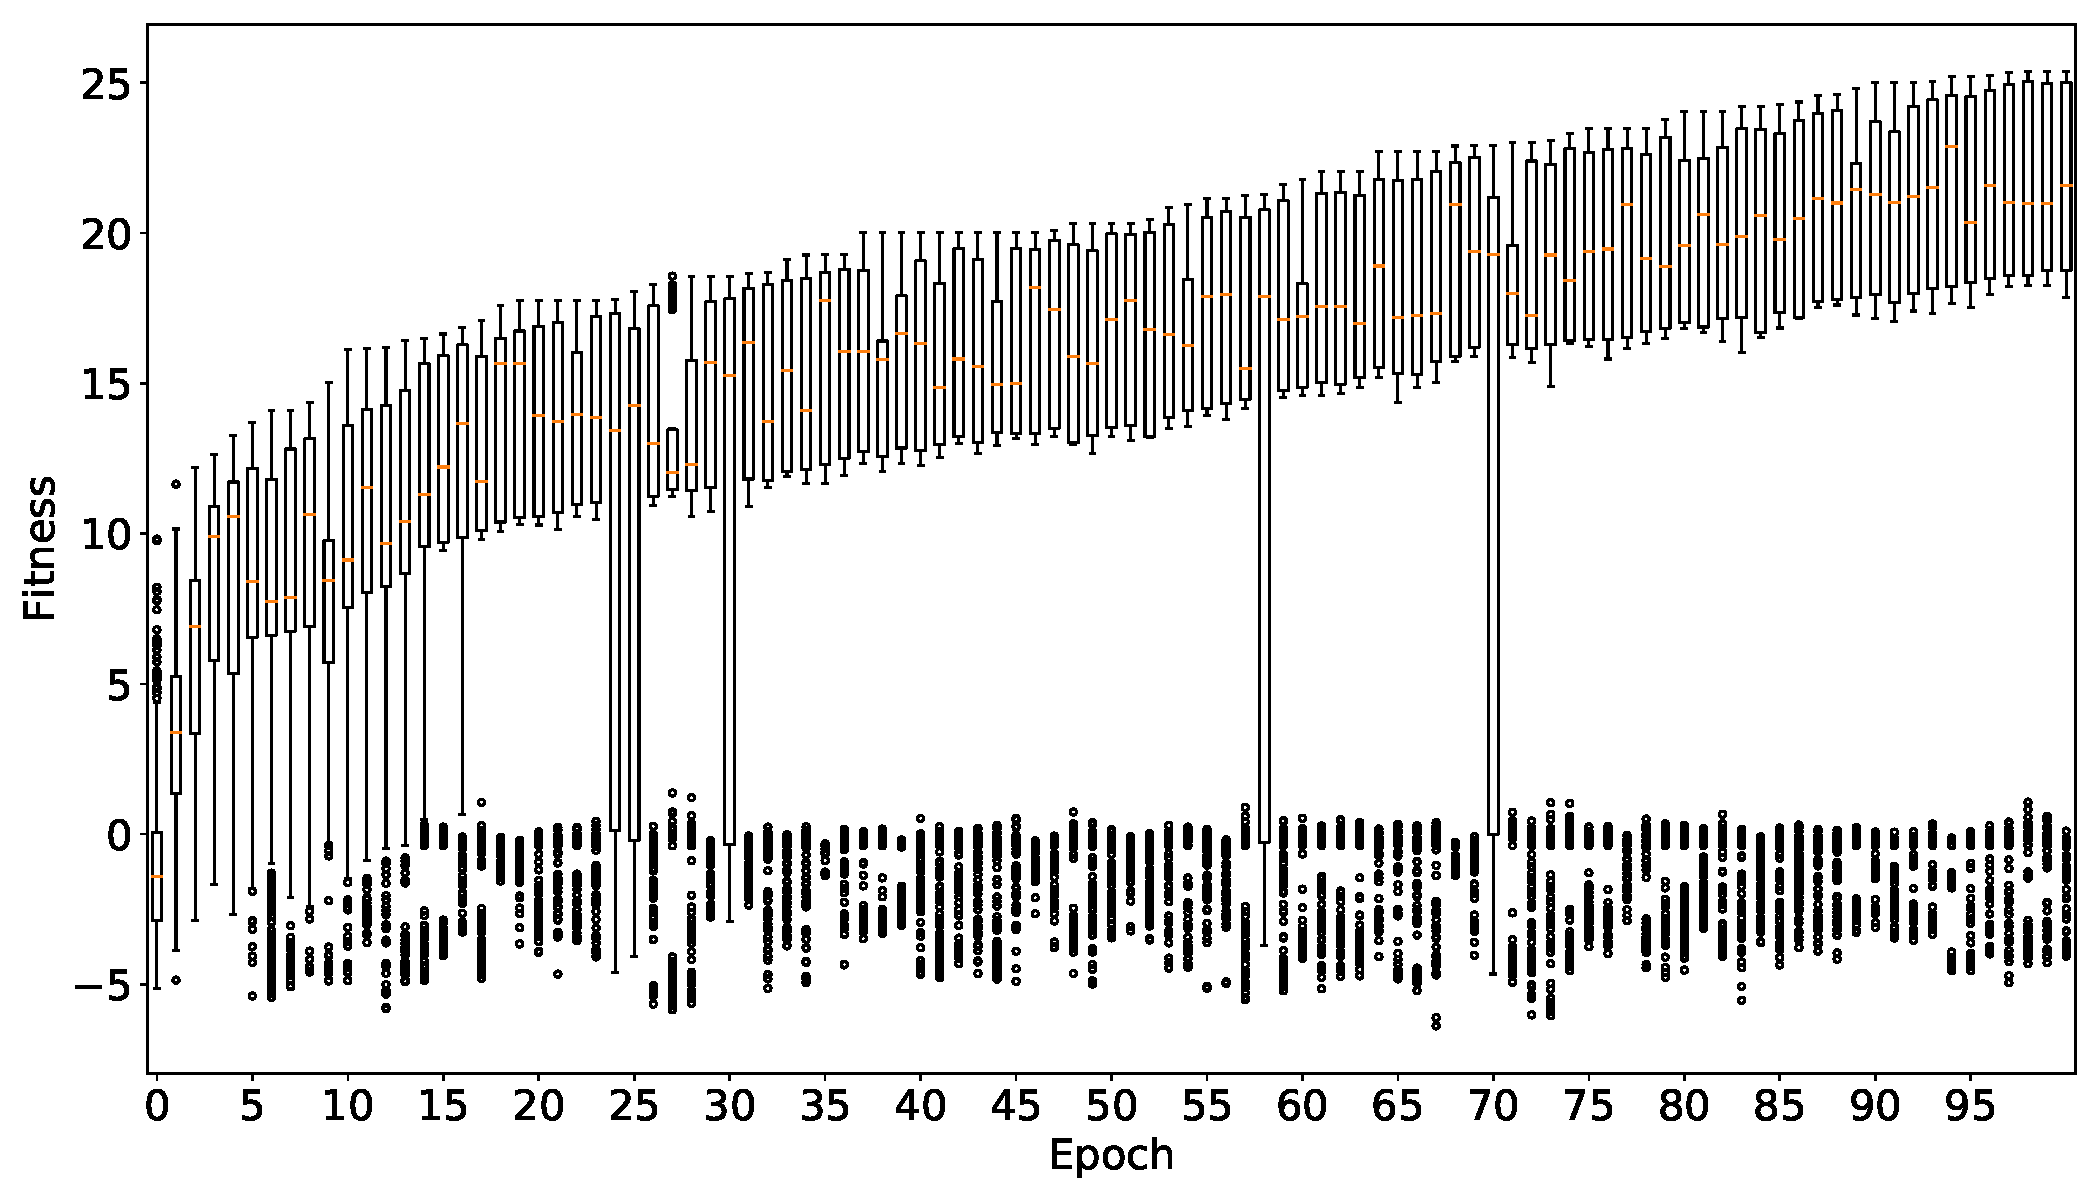
\includegraphics[width=.9\paperwidth]{../img/circle/fitness.pdf}
    }
}

\frame{%
    \makebox[\linewidth]{%
        
\includegraphics[width=.9\paperwidth]{../img/circle/main.pdf}
    }
}


\frame{%
    Given a set of \(k\) \alert{dissimilarity} measures:
    \[
        f_1, \ldots, f_k: \mathbb{R}^n \times \mathbb{R}^n \to \mathbb{R}
    \]

    \alert{Minimise} their sum
}

\frame{%
    \makebox[\linewidth]{%
        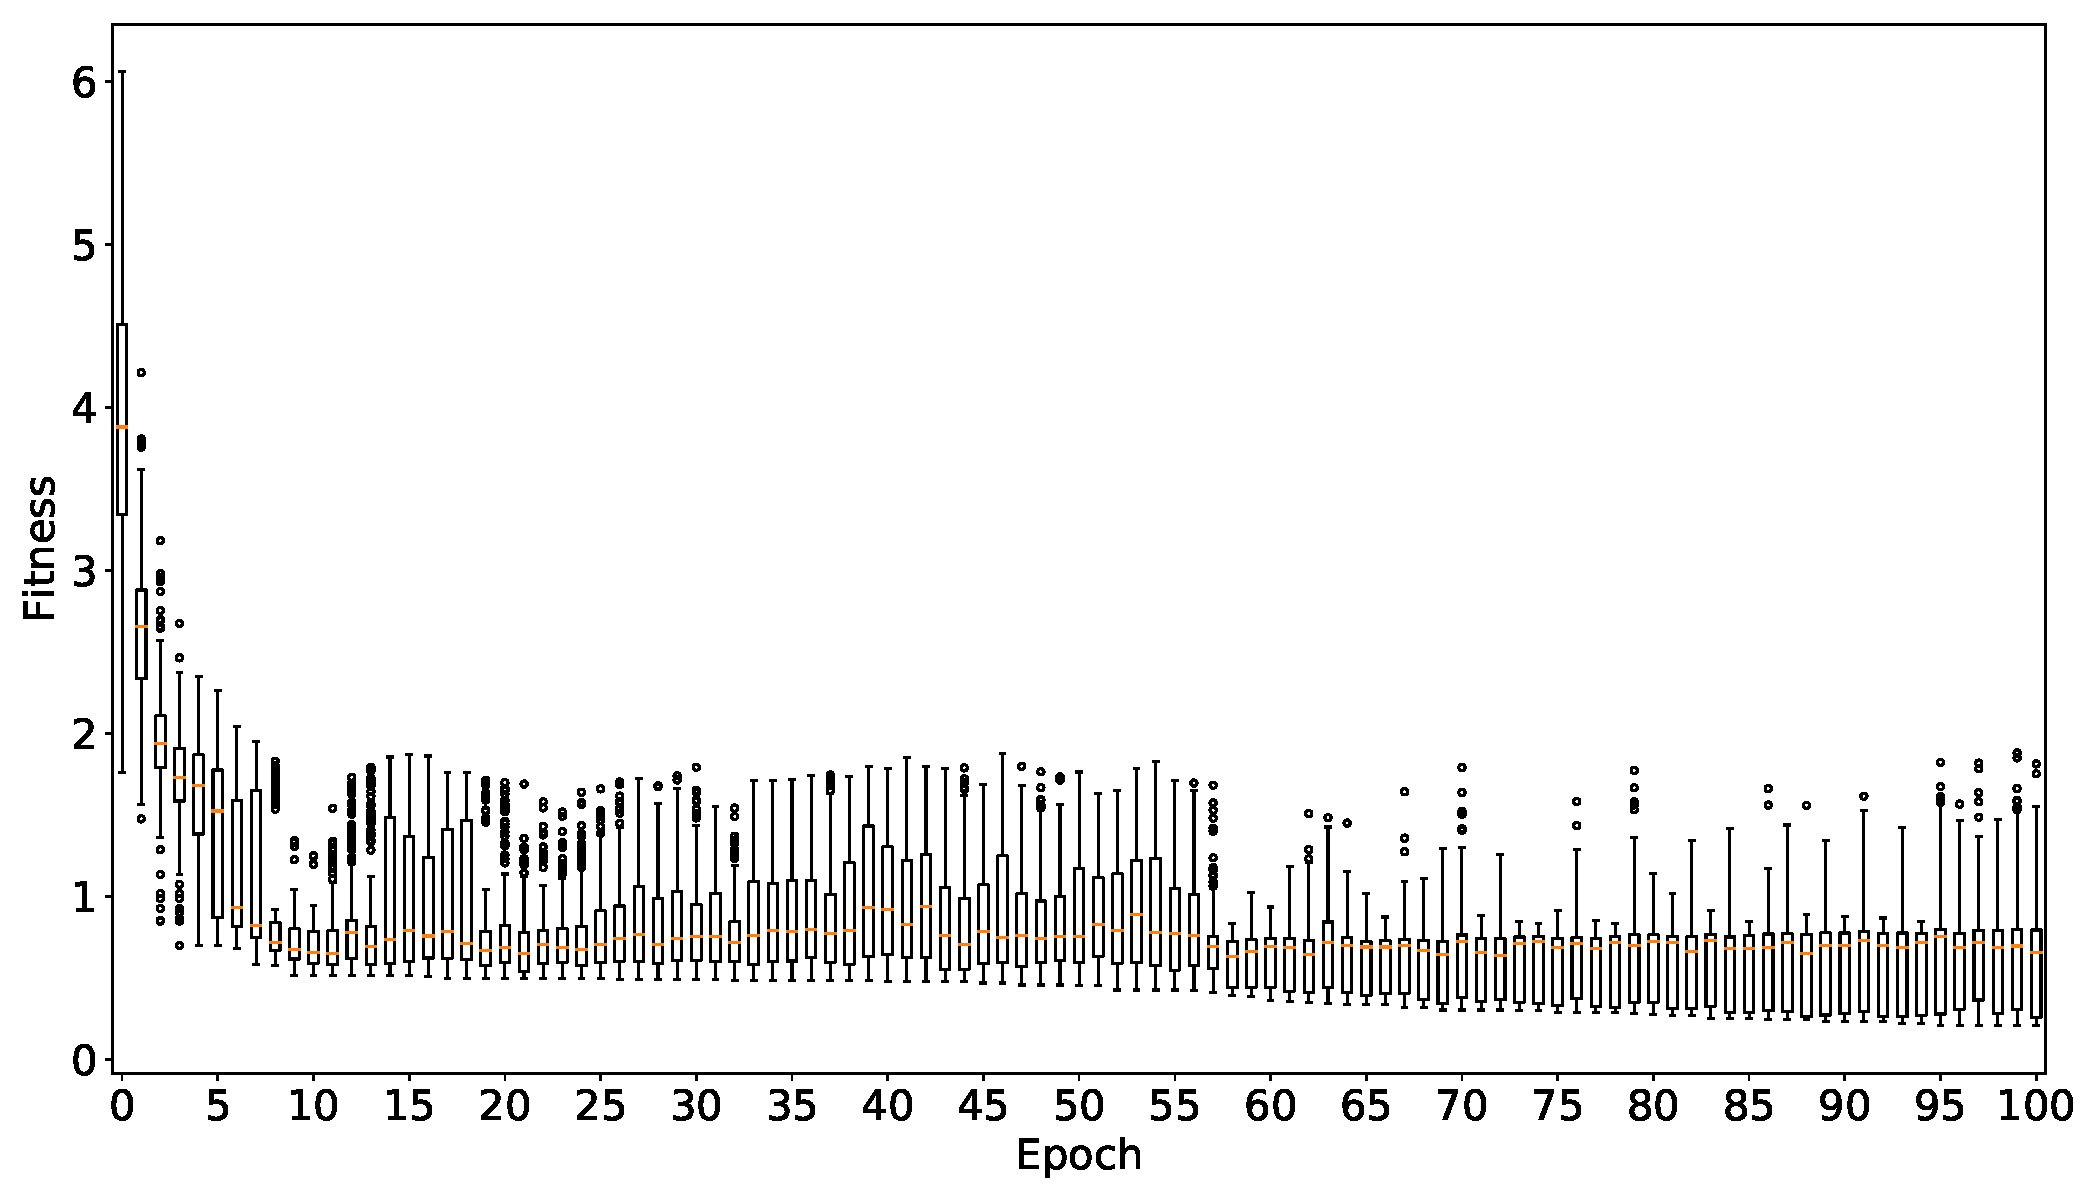
\includegraphics[width=.9\paperwidth]{../img/anscombe/fitness.pdf}
    }
}

\frame{%
    \centering{%
        \(X\) Mean: 5 \hfill%
        \(Y\) Mean: 7 \hfill%
        \(X\) Std.: 4.7 \hfill%
        \(Y\) Std.: 4.1 \hfill%
        Corr.: 0.8
    }\vfill

    \begin{minipage}{\linewidth}
        \hspace*{-30mm}
        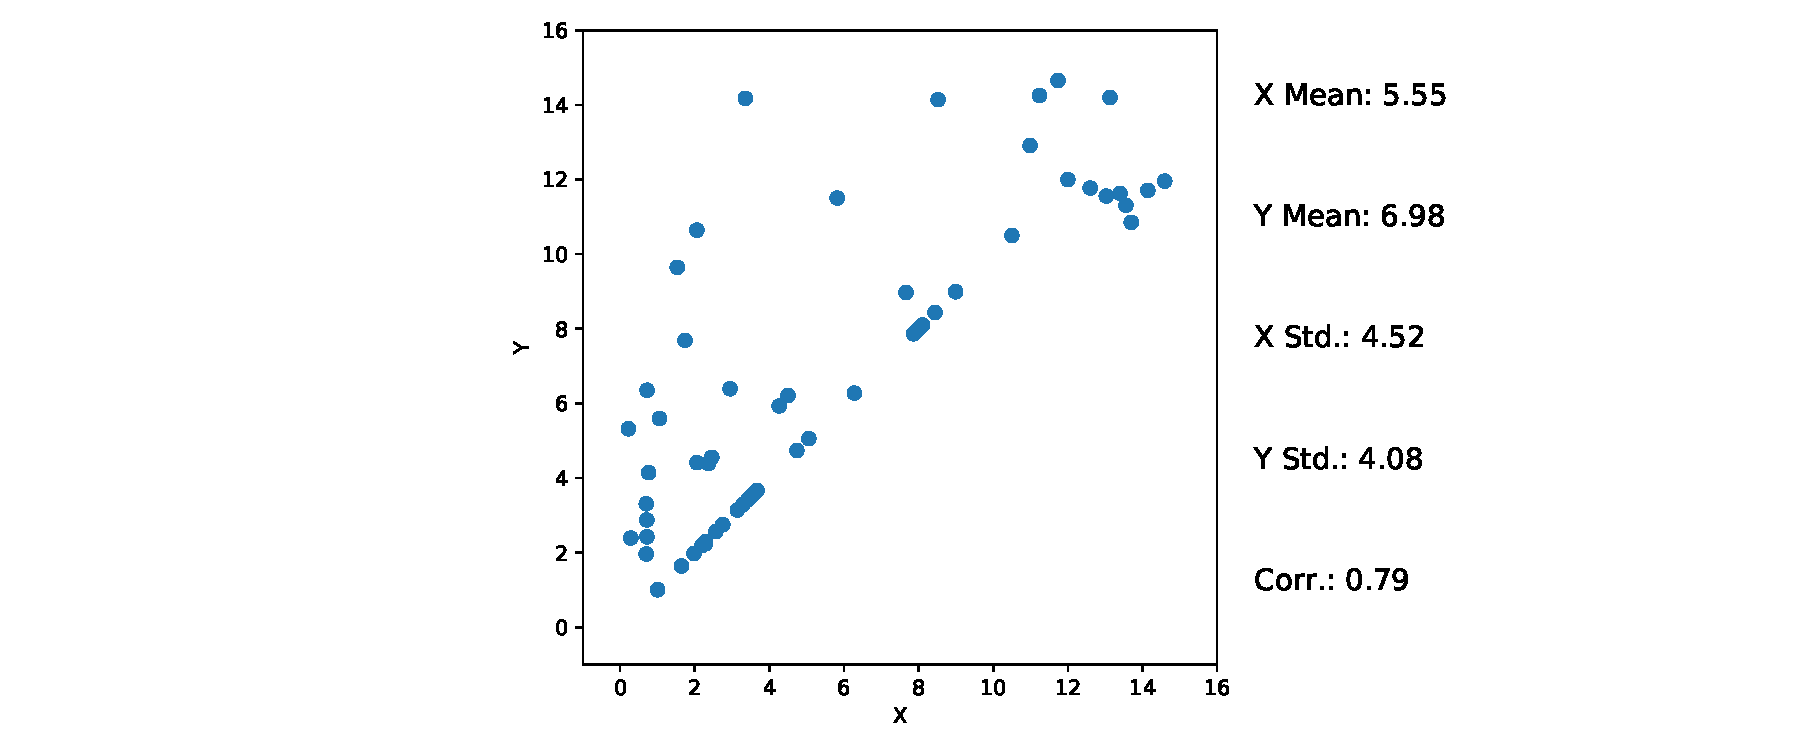
\includegraphics[height=.4\paperheight]{../img/anscombe/best_0.pdf}%
        \hspace*{-30mm}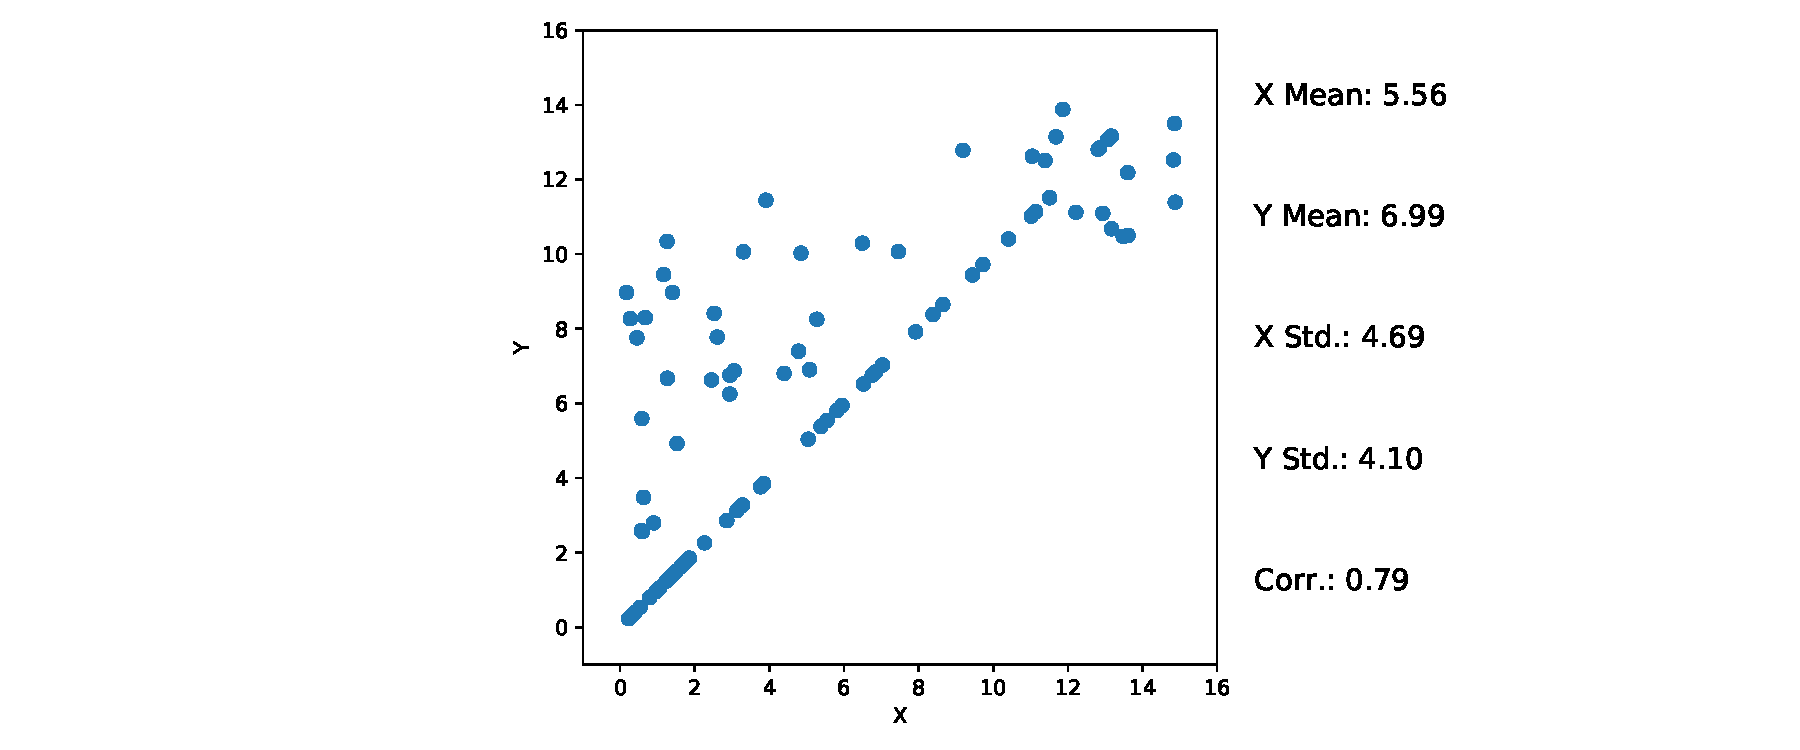
\includegraphics[height=.4\paperheight]{../img/anscombe/best_1.pdf}
    \end{minipage}
    \begin{minipage}{\linewidth}
        \hspace*{-30mm}
        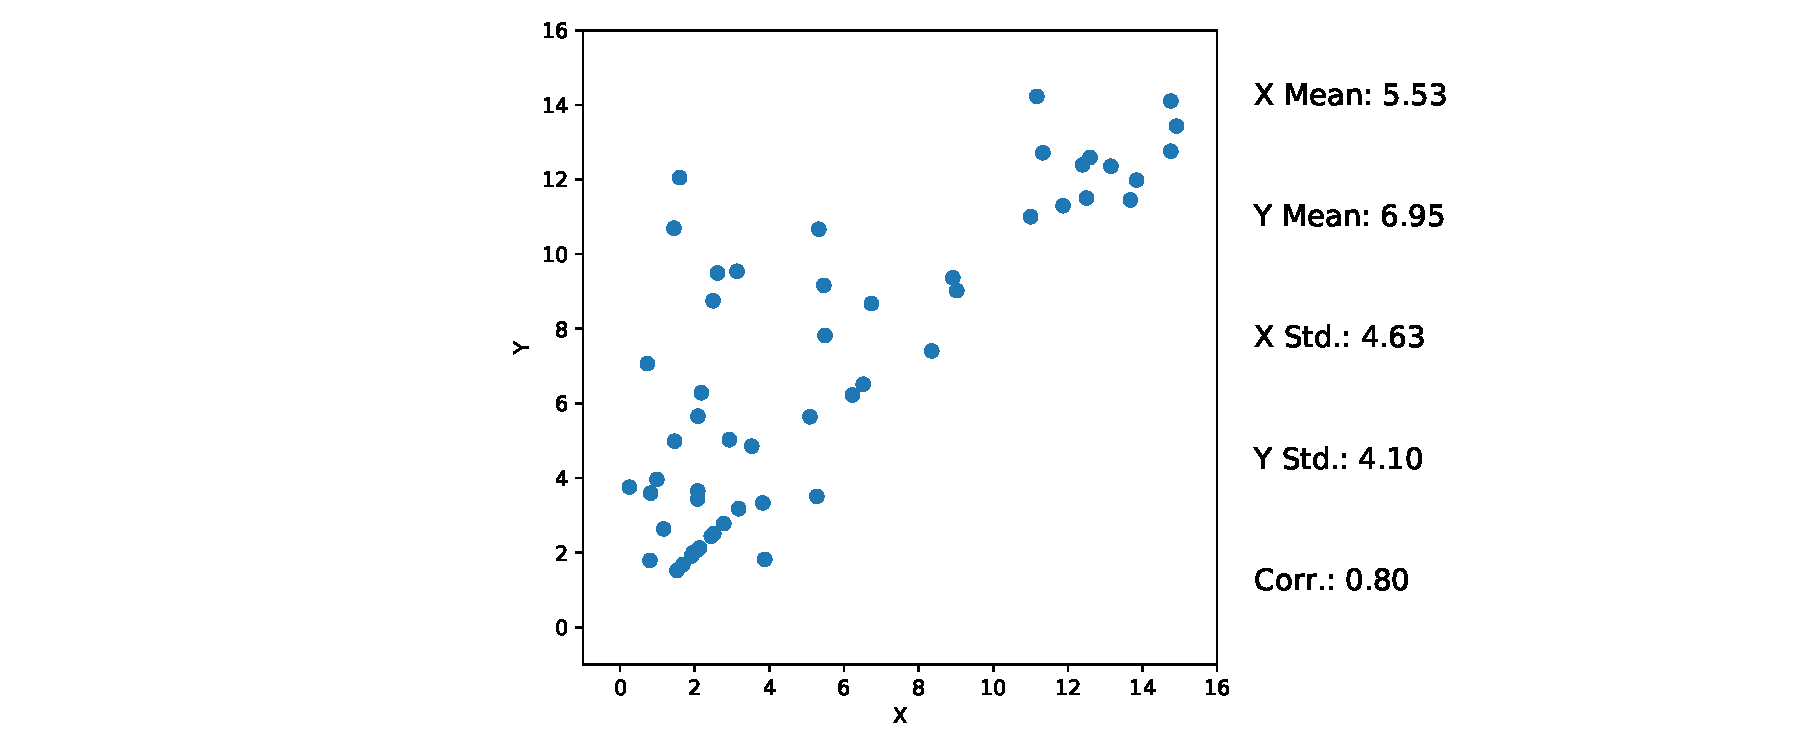
\includegraphics[height=.4\paperheight]{../img/anscombe/best_2.pdf}%
        \hspace*{-30mm}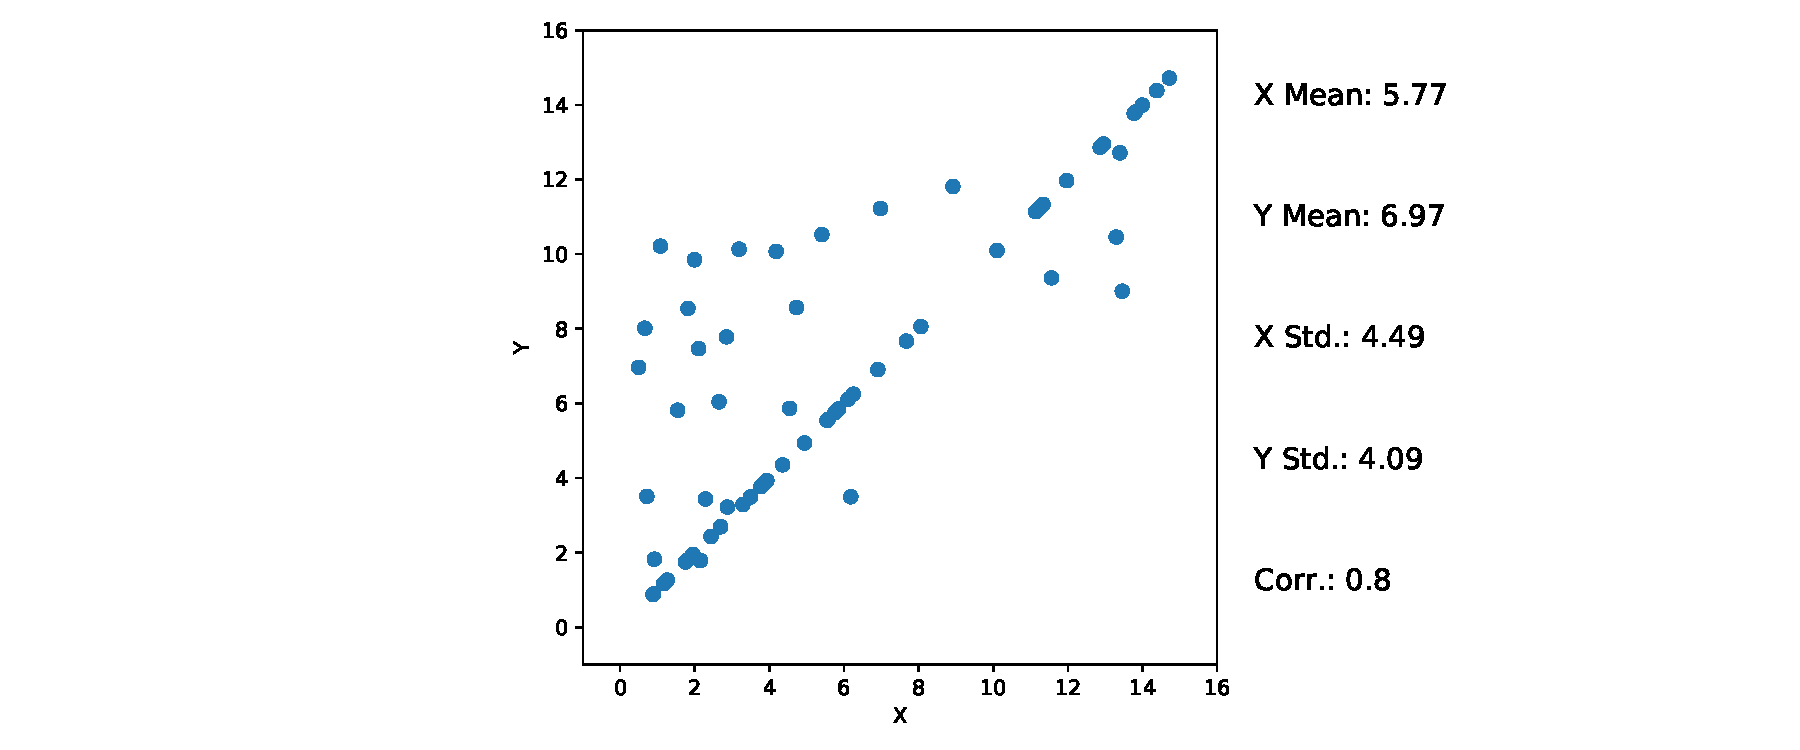
\includegraphics[height=.4\paperheight]{../img/anscombe/best_3.pdf}
    \end{minipage}
}

